\documentclass[UTF8]{ctexart}
\usepackage{amsmath}
\usepackage{listings}
\usepackage{xcolor}
\usepackage{float}
\usepackage{graphicx}
\usepackage{geometry}
\usepackage{enumerate}

\lstset{
    numbers=left, 
    numberstyle= \tiny, 
    keywordstyle= \color{ blue!70},
    commentstyle= \color{red!50!green!50!blue!50}, 
    frame=shadowbox, 
    rulesepcolor= \color{ red!20!green!20!blue!20} ,
    escapeinside=``, 
    xleftmargin=1em,xrightmargin=1em, aboveskip=1em,
    framexleftmargin=2em,
    language = C++
} 
\geometry{left=3cm,right=3cm}
\begin{document}
\begin{figure}
\centering

\includegraphics[scale = 1.5]{title.jpg}
\end{figure}
\title{\Huge数据结构实验报告 \\ [2ex] \begin{Large} 基于改进的Dijstra算法的中文分词实现 \end{Large} }
\author{邱任翔 2018202044}
\date{\today}
\maketitle
\newpage
\tableofcontents
\listoffigures
\newpage
\section{需求分析}
	中文分词(Chinese Word Segmentation) 指的是将一个汉字序列切分成一个一个单独的词。分词就是将连续的字序列按照一定的规范重新组合成词序列的过程。在英文的行文中,单词之间是以空格作为自然分界符的,而中文只是字、句和段能通过明显的分界符来简单划界,唯独词没有一个形式上的分界符。高质量的中文分词是中文文本分析和自然语言处理的基础。\par
	本程序采用了在Dijkstra算法的基础上进行改进的N-最短路径方法。首先根据词典将目标句子构造成有向无环图,每条边代表可能的字词,每条边的权重则是对应再次在词典中的权重(没有则视为无穷大)。则前N短的路径就有理由认为是最有可能的分词方法。该算法的简述如下:\par
\begin{enumerate}
\item 每个结点处记录N个最短路径值,并记录相应路径上当前结点的前驱。
\item 如果同一长度对应多条路径,必须同时记录这些路径上当前结点的前驱,最后通过回溯即可求出N-最短路径。
\end{enumerate}\par
	程序的任务是对用户输入的语段进行中文分词。用户需要输入含有中文字符语段(GB2312编码,可带有特殊字段),并且输入需要输出的前n条最短路径。\par
	程序执行的命令有:\par
\begin{enumerate}[1)]
\item 根据停词表清洗语段中的非中文字符(如标点符号等);
\item 建立词典,并可根据不可分词表修改词典;
\item 根据语段和建立的词典构造DAG;
\item 通过改进的Dijkstra算法求N-最短路径;
\item 根据TF-IDF优化DAG图中的权重;
\item 输出前n条分词结果,并做出词性标注。
\end{enumerate}
\newpage
\section{概要设计}
	为实现上述程序功能,应至少需要两个抽象数据类型,图和索引。\par
\subsection{图的抽象数据类型定义:}
\begin{lstlisting}
ADT Graph{
`数据对象V:是具有相同性质的数据元素的集合。`
`数据关系R:R={<u,v>|P(u,v)∧(u,v∈D)}`
`基本操作:`
CreaeteGraph(&G,V,VR)
`初始条件:V是图的顶点集`
`操作结果:按V和VR的定义构造图G`
DestroyGraph(&G)
`初始条件:图G存在`
`操作结果:销毁图G`
LocateVex(G,u)
`初始条件:图G存在,u和G中有相同的顶点特征`
`操作结果:若G中存在顶点u则返回该顶点在图中位置`
GetVex(G,v)
`初始条件:图G存在,v是G中某个顶点`
`操作结果:返回v的信息`
GetShortestPath(G,st,nd,&Path)
`初始条件:图G存在,st和nd是G中两个顶点`
`操作结果:若st和nd之间存在最短路径,则以Path返回两点之间的一条最短路径`
}ADT Graph
\end{lstlisting}
\subsection{索引的抽象数据类型}
\begin{lstlisting}
ADT Index{
`数据对象V:V是Key和Value以键值一一对应的方式建立一个二维数组`
`数据关系R:R = {(key,value)|key,value∈V}`
`基本操作:`
Init(&I)
`操作结果:初始化索引`
Insert(&I,k,v)
`初始条件:索引I存在,且I中不含k`
`操作结果:向I中插入(k,v)`
Find(&I,k)
`初始条件:索引I存在,且I中含k`
`操作结果:返回key值为key的索引条目的信息`
DestroyIndex(&I)
`初始条件:索引I存在`
`操作结果:销毁索引I`
}ADT Index
\end{lstlisting}
\subsection{程序模块}
\begin{enumerate}[1)]
\item 主程序模块:
\begin{lstlisting}
int main(){
`初始化;`
`接受命令(输入语段以及所需最短路径数目N);`
`处理命令;`
}
\end{lstlisting}
\item 语段清洗模块——根据停词表清洗语段中的非中文字符(如标点符号等);
\item 词典建立模块——建立词典,并可根据不可分词表修改词典;
\item 有向无环图模块——根据语段和建立的词典构造DAG;
\item N最短路径算法模块——通过改进的Dijkstra算法求N-最短路径;
\item TF-IDF模块——根据TF-IDF优化DAG图中的权重;
\item 基于Qt的用户界面。
\end{enumerate}
模块关系图如下:
\begin{figure}[H]
\centerline{
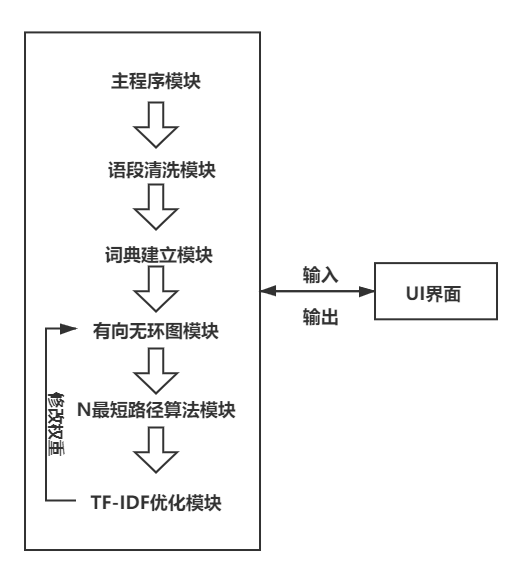
\includegraphics[scale = .6]{part.png}
}
\caption{\textbf{模块关系图}}
\end{figure}
\newpage
\section{详细设计}
\subsection{核心设计}
此处的详细申明为未与界面建立接口,可直接在DOS界面输出时的代码。
1.头文件的申明:\par
\begin{lstlisting}
#include <iostream>
#include <stdlib.h>
#include <string.h>
#include <fstream>
#include<algorithm>
#include<cmath>
#include <map>
#include <vector>
using namespace std;
\end{lstlisting}
2.基本类型的定义:\par
\begin{lstlisting}
#define INF 0x3f3f3f3f
typedef struct Table{`//DAG每个结点所存储的信息`
    int num;`//源点到该结点最短路径的序号`
    double length;`//源点到该节点的最短路径`
    int pre[2];`//pre[0]表示到该节点的最短路径的前驱的下标,pre[1]表示该前驱中对应的前n短路径的序号`
}Info;
typedef struct Keyword{`//TF-IDF优化时需要的关键词,负责方便记录和修改在语段中出现的词典的词`
    string key;
    int i;`//对应DAG中的下标`
    int j;
}Keyword;
typedef struct Word{`//每个词的结构体,有权重和词性两种属性`
    double weight;
    string kind = "unknown";`//初始化词性为unknown`
}Word;
vector<Keyword>keywords;`//存储关键词的数组`
map<string,Word>dict;`//存储词典的索引表,方便通过查找字串找到对应字典的权重`
}
vector<string> stopwords;`//可以自行添加停词表`
\end{lstlisting}
3.图的基本操作:\par
\begin{lstlisting}
vector<vector<Word>> BuildGraph(string &s)
`//根据词典和语段构造DAG,用邻接矩阵来表示,i->j边代表语段从i+1个字开始的j-i个字符`

`算法如下:`
vector<vector<Word>> BuildGraph(string &s){
    int i,j,l;string ps;Word non;Keyword Key;non.weight = INF;
	 l = s.length()/2+1;
    vector<vector<Word>>graph(l,vector<Word>(l,non));`//邻接矩阵的初始化`
    for(i = 0;i < l;i++){
        for(j = i;j < l;j++){
            if(i == j)graph[i][i].weight = 0;
            else{
                ps = s.substr(2*i,2*(j-i));`//选取字符串的子串赋给邻接矩阵`
                cout<<ps;
                graph[i][j].weight = SearchInDict(ps).weight;
                if(graph[i][j].weight < INF){`//记录下关键词`
                    Key.i = i;Key.j = j;
Key.key = ps;
keywords.push_back(Key);
                }
                graph[i][j].kind = SearchInDict(ps).kind;
            }
        }
    }
    return graph;
}
\end{lstlisting}
4.索引的基本操作:\par
\begin{lstlisting}
void GetDict()
`//根据读取的文件创建词典和不可分词表`
Word SearchInDict(string &s)
`//根据字符串查找词典中对应的权重`

`部分操作的算法如下:`
void GetDict(){
`//打开文件,词典文件指针为infile,不可分词表文件指针为specialwords`
    string s,cn,kind;Word c;const char * w;
    unsigned long long pos;
    while(getline(infile,s)){`//采用字符串分割`
        pos = s.find(" ");
        cn = s.substr(0,pos);
        s.erase(0,pos+1);
        pos = s.find(" ");
        w = s.substr(0,pos).c_str();
        c.weight = atoi(w);`//将词典中词频有字符串转化为浮点数类型`
        kind = s.substr(pos+1);
        c.kind = kind;
        dict.insert(pair<string,Word>(cn,c));
    }
    while(getline(specialwords,s)){`//向创建好的词典中添加停用词`
        Word sp;
        sp.weight = 0;
        map<string,Word>::iterator iter;
        iter = dict.find(s);
        if(iter != dict.end())iter->second.weight = 0;`//如果该词在词典中有,则将其权重修改为0`
        else dict.insert(pair<string,Word>(s,sp));
    }
	while(getline(stop,s)){
        stopwords.push_back(s);
    }
}
Word SearchInDict(string &s){`//根据字符串查找词典中对应的权重`
    Word non;
    non.weight = INF;
    map<string,Word>::iterator iter;
    iter = dict.find(s);
    if(iter != dict.end())return iter->second;
    else return non;
}
\end{lstlisting}
4.主程序和其他伪码算法
\begin{lstlisting}
int main()
{
	`输入命令`
	 GetDict();
    Wash(s);
    G = BuildGraph(s);
    if(m)TF_IDF(s,G);
    Dijkstra(G,n,l,s);
	 rerurn 0;
}
void Wash(string &s){`//对语段进行清洗,除去无用字段`
    int pos = 0;
    for(int i = 0;i < stopwords.size();i++)
    {
        for(pos = s.find(stopwords[i]);
		  pos != string::npos;
		  pos = s.find(stopwords[i])){
            s.erase(pos,2);
        }
    }
}
void TF_IDF(string &s,vector<vector<Word>> &G){`//TF-IDF优化`
    int index = 0;int count = 0;int n = keywords.size();
    for(int i = 0;i < n;i++)
    {
        index = 0;count = 0;
        for(index = s.find(keywords[i].key,index);
index != string::npos;
index = s.find(keywords[i].key,index)){
            count++;
            index = index + keywords[i].key.size();
        }
        G[keywords[i].i][keywords[i].j].weight = 
log(SearchInDict(keywords[i].key).weight)/count;
`//根据优化后结果修改DAG图的数据`
    }
}
int cmp(const Info &a,Info &b){`//方便使用sort函数,根据Info中路径长度进行排序`
    return a.length<b.length;
}
void NMin(vector<Info> &can,int n){`//对每个结点信息进行整理,只保留源点到其的前n条最短路径`
    vector<Info> newcan;
    sort(can.begin(),can.end(),cmp);`//排序`
    if(can.size() > n)can.resize(n);
    for(int i = 0;i < can.size();i++){
        if(i!=0 && can[i].pre == can[i-1].pre)can.erase(can.begin()+i);
`//如果出现重复路径,则删除其中一个`
            else can[i].num = i;
    }
}
void Print(vector<vector<Info>> &tables,vector<vector<Word>> &G,
string &s,int l,int n){`//对分词结果的打印`
    int k,i,j,t;
    string as,ss;`//as存储词性,ss存储分词后的语段`
    for(k = 0;k < n;k++){
        ss = s;as.clear();t = l-1;
        cout<<"`第`"<<k+1<<"`条最短路径`:";
        for(i = tables[l-1][k].pre[0],j = tables[l-1][k].pre[1];
i != 0;
i = tables[t][j].pre[0],j = tables[t][j].pre[1]){
            as = "-" + G[i][t].kind + as;`//词性标记`
            ss.insert(2*i,"/");`//在语段中插入“/”,达到分词的目的`
            t = i;
        }
        as = G[0][t].kind + as;
        cout<<ss<<"`词性标记`:"<<as<<endl;
    }
}
void Dijkstra(vector<vector<Word>> &G,int n,int l,string &s){
`//在Dijkstra算法基础之上进行改进`
    int k;
    vector<vector<Info>> tables(l);`//二维的table数组代表每个结点存储的信息`
    vector<Info> table(n);`//table存储每个结点的信息,且每个table最多存储n条最短路径`
    tables[0].push_back({0,0,{0,0}});`//初始化`
    for(int i = 1;i < l;i++){
        k = 0;
        for(int j = 0;j < i;j++){
            if(G[j][i].weight < INF){
                for(int q = 0;q < tables[j].size();q++){
                    double ll = tables[j][q].length + G[j][i].weight;
`//每一个结点的路径是基于源点到前驱的最短路径与该点到前驱路径相加`
                    tables[i].push_back({k,ll,{j,q}});
                    k++;
                }
            }
        }
        NMin(tables[i],n);
    }
    Print(tables,G,s,l,n);
}
\end{lstlisting}
5.函数调用关系图
\begin{figure}[H]
\centerline{
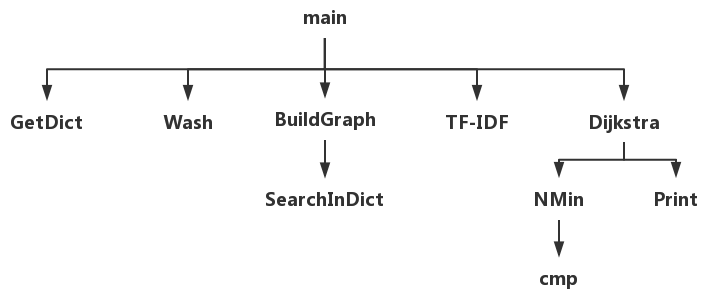
\includegraphics[scale = .6]{relation.png}
}
\caption{\textbf{函数调用关系图}}
\end{figure}
\newpage
\subsection{界面设计}
1.头文件的申明\\
mainwindow.h\par
\begin{lstlisting}
#ifndef MAINWINDOW_H
#define MAINWINDOW_H

#include <QMainWindow>
#include <iostream>
using namespace std;
namespace Ui {
class MainWindow;
}

class MainWindow : public QMainWindow
{
    Q_OBJECT

public:
    explicit MainWindow(QWidget *parent = nullptr);
    ~MainWindow();
private slots:
    void on_pushButton_clicked();`//界面上的两个按钮`
    void on_pushButton_2_clicked();
private:
    Ui::MainWindow *ui;
};
#endif // MAINWINDOW_H
\end{lstlisting}
wg.h
\begin{lstlisting}
#ifndef WG_H
#define WG_H
#include <vector>
#include <QString>
using namespace std;
class wg
{
public:
    wg();
    vector<QString>Run(string&,int,int);`//核心程序与界面的接口,在原来main函数基础之上改`
};

#endif // WG_H
\end{lstlisting}
2.主程序\\
mainwindow.cpp
\begin{lstlisting}
#include "mainwindow.h"
#include "ui_mainwindow.h"
#include "wg.h"
#include <iostream>
#include <QString>
#include <QTextCodec>
#include <string.h>

using namespace std;

MainWindow::MainWindow(QWidget *parent) :
    QMainWindow(parent),
    ui(new Ui::MainWindow)
{
    setFixedSize(500,350);
    ui->setupUi(this);
}

MainWindow::~MainWindow()
{
    delete ui;
}

void MainWindow::on_pushButton_clicked()`//运行按钮`
{
    wg W;
    string in;
    vector<QString>out;
    int num;
    int flag = 0;
    QString st;
    st = ui->plainTextEdit->toPlainText();
    QTextCodec* pCodec = QTextCodec::codecForName("gb2312");`//将输入的字符从UTF-8转gb2312`
    QByteArray arr = pCodec->fromUnicode(st);
    in = arr.data();
    num = ui->spinBox->value();
    if(ui->checkBox->isChecked()){
       flag = 1;
    }
    out = W.Run(in,num,flag);
    for(int i = 0;i < out.size();i++)
    {
        ui->textBrowser->append(out[i]);`//显示输出结果`
    }
    ui->textBrowser->append("$\backslash$n");
}

void MainWindow::on_pushButton_2_clicked()`//清屏按钮`
{
    ui->textBrowser->clear();
}
\end{lstlisting}
wg.cpp(此处相当于核心设计中的代码,因此只需要修改相关输入和输出的函数即可)
\begin{lstlisting}
vector<QString> wg::Run(string &s,int n,int m)
{
    int l;
    GetDict();
    Wash(s);
    l = s.length()/2 + 1;`//计算构造DAG的节点数`
    vector<vector<Word>> G(l,vector<Word>(l));
    G = BuildGraph(s);
    if(m)TF_IDF(s,G);
    return  Dijkstra(G,n,l,s);
}
vector<QString> Print(vector<vector<Info>> &tables,vector<vector<Word>> &G,string &s,int l,int n){`//对分词结果的打印`
	`//核心设计中print函数略`
        final = ss+`"$\backslash$n词性标记:"`+as 
+`"$\backslash$n路径长度:"` + to_string(tables[l-1][k].length);
        QTextCodec* pCodec = QTextCodec::codecForName("gb2312");
`//中文编码的转换先将gb2312转Unicode再转UTF-8`
        QString qstr = pCodec->toUnicode(final.c_str(), final.length());
        qs.push_back(qstr);
    }
    return qs;
}
\end{lstlisting}
main.cpp
\begin{lstlisting}
#include "mainwindow.h"
#include <QApplication>

int main(int argc, char *argv[])
{
    QApplication a(argc, argv);
    MainWindow w;
    w.show();
    return a.exec();
}
\end{lstlisting}
\section{设计和调试分析}
\subsection{设计分析}
	1.在实现了实验报告中的基本功能和拓展功能之外,本文针对中文分词还做了以下改进:\par
\begin{enumerate}[1)]
\item 添加了对输入语段进行预处理的功能,可以去除非中文字符或其他无意义的字词;
\item 可以自行添加不可分词表
\item 可以启用/关闭TF-IDF模块,对DAG的权重进行优化;
\item 输出分词结果的同时对分词的词性进行标记(充分利用词典信息)。
\end{enumerate}\par
	以上功能的设计是让该中文分词程序更具实用性和操作性。\par
	2.关于文中的N-最短路径算法,其本质是基于Dijkstra算法基础上的贪心算法。原有的Dijkstra算法每次更新后的路径都是源点到该点的最短路径,那么一直迭代到终点,就自然是源点到终点的最短路径。那么在此基础之上扩展,每次都找到源点到当前点的前n条最短路径,下一个点的前n条最短路径是在源点到前一个点前n条最短路径的基础之上进行迭代,最后即可找到源点到终点的前n条最短路径。\par
	3.关于该算法的复杂度分析:一个含有n个中文字符的语段,其构造出的DAG的邻接矩阵为$(n+1)*(n+1)$,故空间复杂度为o($n^2$)。而对于时间复杂度,该语段最多可划分出(n+1)n/2个字词,不妨设每个单字作为字典中出现的词的末字的平均次数为k,此时k也代表了每个结点里面存储信息的平均数目,则时间复杂度为o($(n+1)nk/2$),即o($kn^2$)的空间复杂度。\par
	4.在程序实现的过程中,本文使用了通过string类的库函数完成字符串处理部分,并且使用STL中的vector容器实现了对所有顺序表以及图的定义,通过map容器定义索引,这些模板类的运用大大减少了空指针、内存泄漏等问题,并且实现数据结构和算法的分离,提高了开发的效率,并使代码的可读性增强。\par
	5.由于本来就是用Qt做的C++程序,索性直接做了一个可视化界面,方便用户更加容易操作。
\subsection{调试分析}
	1.在编写N-最短路径算法时(Dijkstra函数和NMin函数),在求源点到每个结点前n短路径的过程时错误地直接用等于号赋值修改table的信息,未考虑空间分配等问题,耗费了部分时间。\par
	2.本文在实现TF-IDF优化的过程中,发现词典并未提供其语料库文档的总数,无法求其IDF(逆文档频率) = lg((语料库文档总数)/(包含该词的文档数+1)),但该算法的本质使区分一篇语段中的关键词,帮助我们将其更加明显地划分出来。那么如何判断一个词是不是关键词呢?根据该方法的思想是如果该词在文章中出现的词频越大,而语料库中出现的数量越少(取对数是为了矫正频数差别过大导致的误差),则该词就越有可能是关键词。在理解这样思想的基础下,移植到中文分词程序中,即DAG中代表词的边的权重应针对此进行修正,即该词所在边的权重和语料库(词典)的词频数成正比,和语段的词频数成反比。文章采用的处理是:权重 = ln(语料库的词频数)/语段中该词的词频数;这种修正在一些测试案例中取得了较好的效果。\par
	3.在最后输出时,本来是打算有和输出最短路径一样,用递归来进行回溯来输出最后分词结果。但分词与原语段相比仅有分词号" $\backslash$"的差别,且通过回溯法最先求得的是最后一段路径,如果在此进行插入分词号,不会影响前面字符的位置,所以作者直接使用插入" $\backslash$"完成分词。\par
	4.在测试时,作者试图批量运行测试案例时发现出现内存泄露而导致程序报错的问题,经检查发现未在最后释放STL容器占用的空间,这在测试单一案例时并无问题,只有重复运行函数时才会出现。在最后调用容器的clear()函数得以解决。\par
	5.在设计操作界面时遇到了很多意想不到的问题。因为已经完成了对核心代码的测试,而在与界面进行接口时程序总是在输入后运行时发生crashed,在Debug的过程中,发现最早连DAG图的节点个数l都是错误的,这才意识到可能是中文编码出现了问题。尽管修改了Qt中文本编辑器的编码为GB2312,但这只会让其在DOS环境下运行不会出错,而Qt的图形界面中使用的QString仍然是UTF-8的编码。所以在输入和输出时需要进行转码。何况Qt并不支持GB2312和UTF-8的直接转换,所以我以Unicode编码为中转,利用Qt自带的QTextcodec库完成了编码的转换,程序得以正常运行。\par
	6.本程序最后采用的均是相对路径的文件读取方法,而在测试时却一直采用绝对路径读取文件。是因为Qt在编译程序时会生成一个“影子”程序进行运行而不直接编译源程序,所以无法使用相对路径。当然也可以考虑将文件加入Qt的resource,但这样使用QFile读文件又会涉及到文件编码的处理问题,便舍弃了这种做法。\par
	7.为方便在未安装Qt环境的电脑也能运行该程序,通过Qt的windeployqt指令对程序进行打包处理,只需直接运行执行文件即可使用。
\newpage
\section{测试结果和分析}
	为方便批量读取文件和显示结果,测试均在DOS界面进行,测试的案例主要分为三类:
\begin{enumerate}
\item 在不作TF-IDF优化下的简单的基本语句;
\item 添加不可分词表前后的语句;
\item 启用优化后的语句对比;
\end{enumerate}\par
	默认输出前5条最短路径,并输出最后一个结点的存储的信息(table),其第二列的浮点数代表分词的词频相加,即该条分词路径的长度。
\subsection{在不作TF-IDF优化下的简单的基本语句}
\begin{figure}[H]
\centerline{
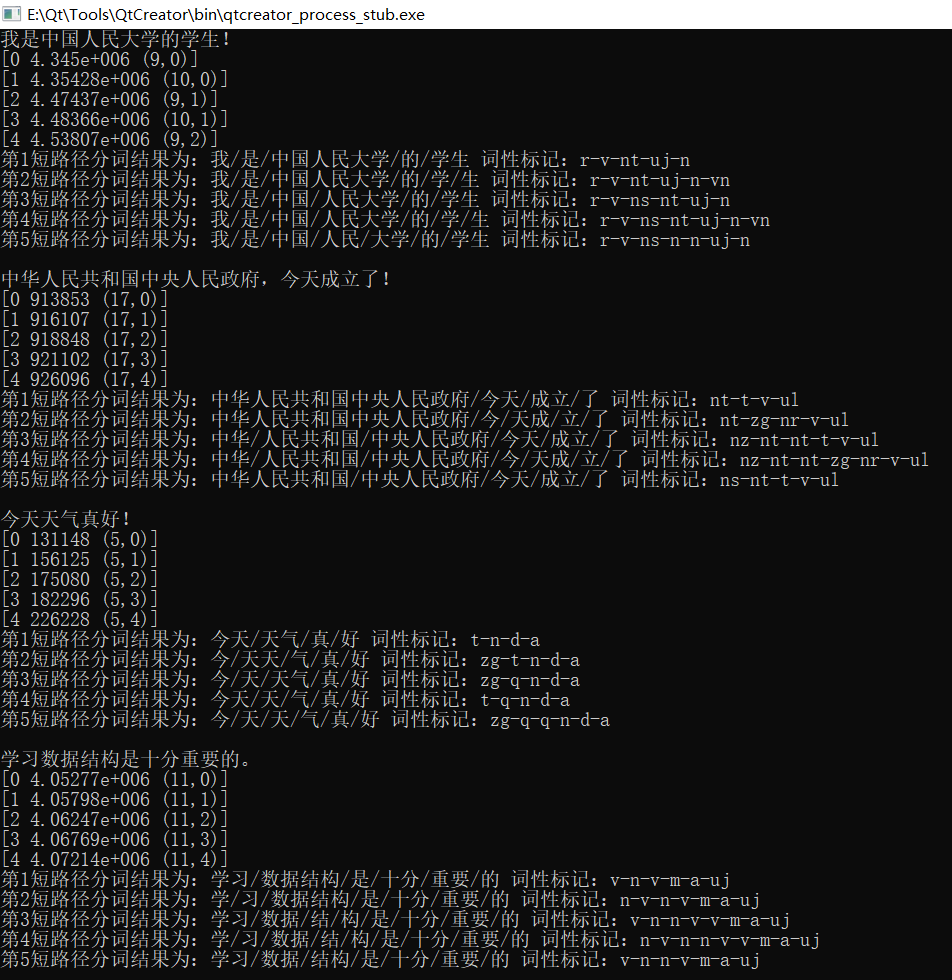
\includegraphics[scale = .5]{test1.png}
}
\caption{\textbf{测试1}}
\end{figure}
	可以看出在程序会自动去除停词表中的标点符号后再进行分词,在输入这些混淆性较小的基本语句时,未优化情况下也会有较好的分词效果。
\subsection{添加不可分词表前后的语句}
在添加不可分词表前(测试2.1),由于输入的语段中含有部分语料库中没有的字词,分词往往达不到预期的效果。\par
添加不可分词表后(测试2.2),相当于向字典中添加了这些权重为0的词,则在分词的过程中便会将这些词视为一个整体。
\begin{figure}[H]
\centerline{
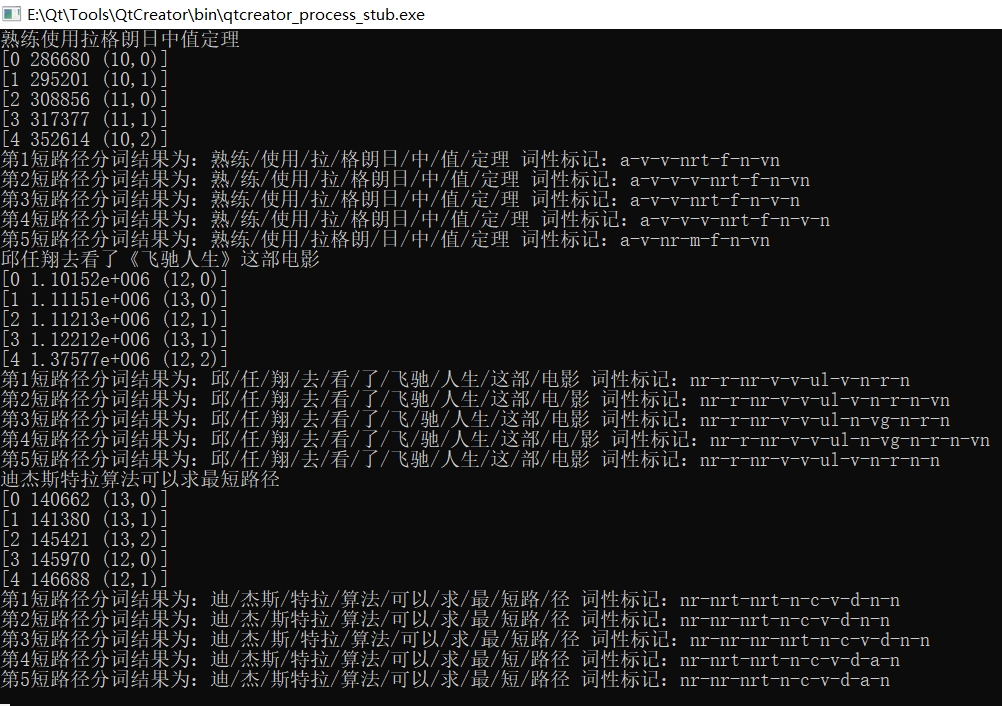
\includegraphics[scale = .5]{test2.png}
}
\caption{\textbf{测试2.1}}
\end{figure}
\begin{figure}[H]
\centerline{
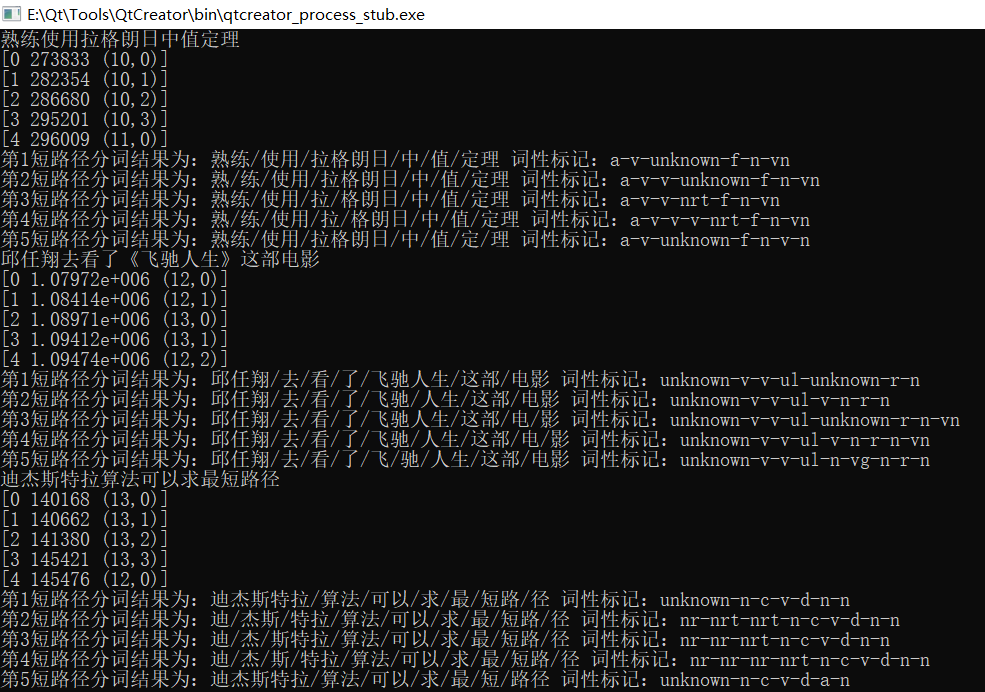
\includegraphics[scale = .5]{test2-1.png}
}
\caption{\textbf{测试2.2}}
\end{figure}
\subsection{启用优化后的语句对比}
在遇到一些特殊的容易发生分词歧义的句子时,未经TF-IDF优化的算法由于受到某些词频较大的字词(高权重)的影响,最合理的分词不一定是路径最短的,而优化的一个取对数过程其实就是相当于对这一差异的矫正,在保持单调性不变的情况下,减小了词频之间的差距,使可能的分词结果可以出现在N-最短路径中。\par
以图示例子可以看出,在启动优化后,分词的结果也更加多样化,最短路径的合理性也有所增加。
\begin{figure}[H]
\centerline{
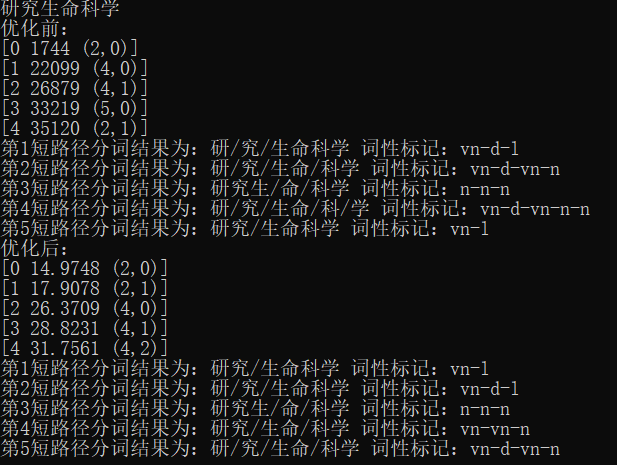
\includegraphics[scale = .6]{test3.png}
}
\end{figure}
\begin{figure}[H]
\centerline{
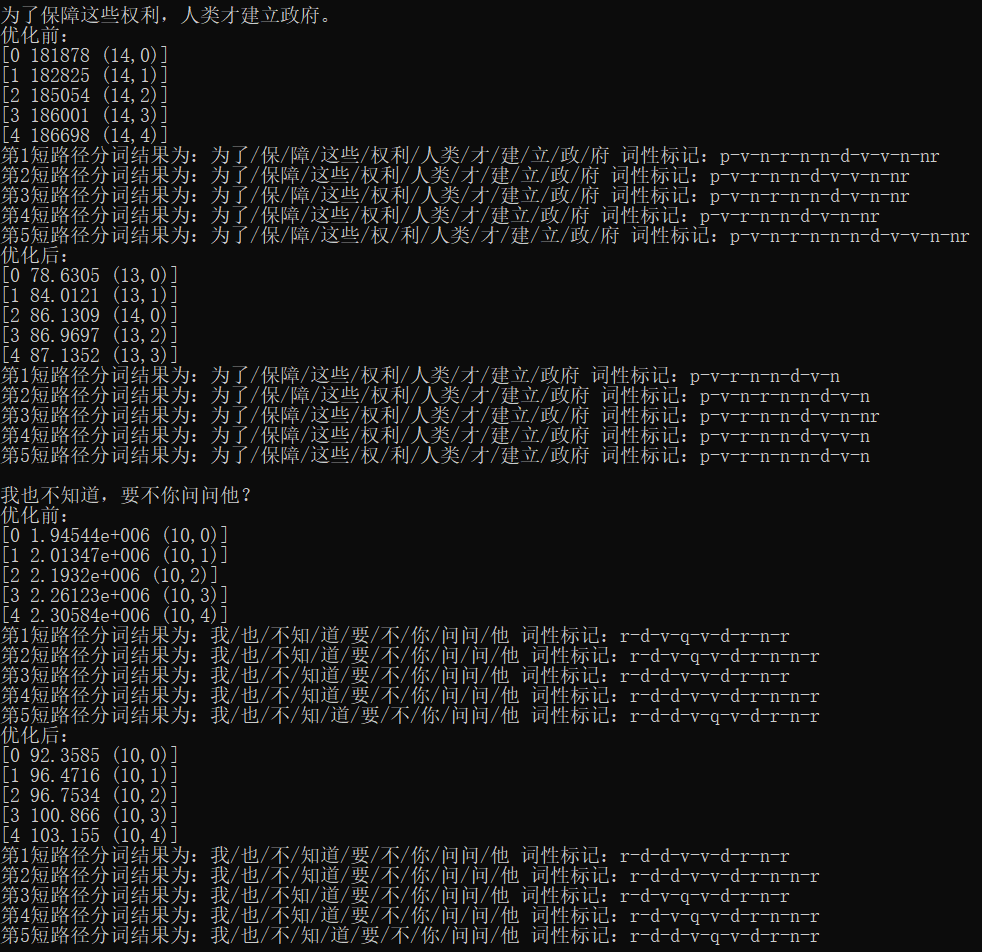
\includegraphics[scale = .5]{test3-3.png}
}
\caption{\textbf{测试3}}
\end{figure}
\newpage
\section{总结}
	1.本程序文件分有界面和无界面两份,分别在Qt和DOS环境中运行(未装Qt也可运行可执行文件),其中Qt中可执行文件为可执行文件夹中的word\_segment\_final.exe,C++中为main.exe;\par
	2.进入程序前,可以自行修改文件夹中的停词表和不可分词表以及词典,进入程序后,按照提示输入所需进行分词的语段以及后续操作即可;\par
3.C++程序运行完毕后会自动重新运行,即可输入下一个分词的语段,而Qt可以任意更改,点击运行即可将每次的结果都输出,也可选择清屏清空当前记录。\par
\begin{figure}[H]
\centerline{
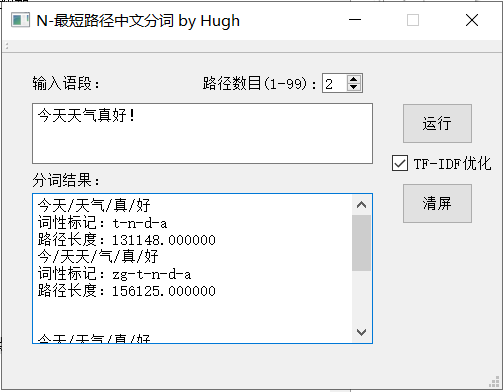
\includegraphics[scale = .8]{ui.png}
}
\caption{\textbf{Qt用户界面}}
\centerline{
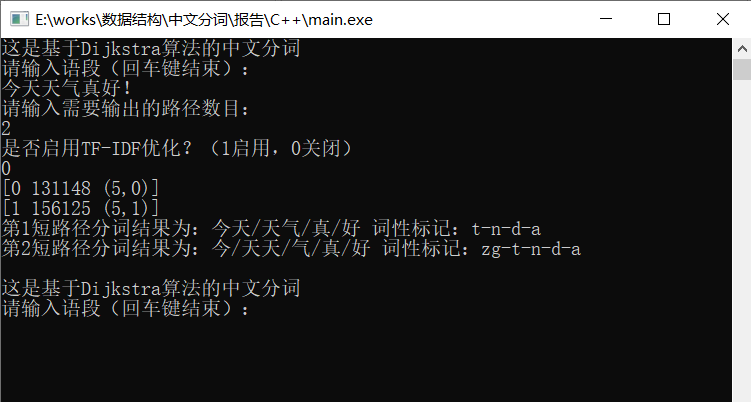
\includegraphics[scale = .7]{ui2.png}
}
\caption{\textbf{DOS用户界面}}
\end{figure}
\newpage
\section{附录}
文件名清单:
C++文件:
\begin{itemize}
\item main.cpp //源程序代码
\item main.exe //封装后程序
\item dict\_gb2312.txt //词典文本
\item stopwords.txt //停词表文本
\item specialwords.txt //不可分词表文本
\end{itemize}\par
Qt中程序文件:
\begin{itemize}
\item main.cpp //主程序代码
\item mainwindow.h //界面类头文件
\item mainwindow.cpp //界面类的实现
\item wg.h //核心类头文件
\item wg.cpp //核心类代码
\item word\_segment\_final.pro //Qt项目文件
\item dict\_gb2312.txt //词典文本
\item stopwords.txt //停词表文本
\item specialwords.txt //不可分词表文本
\end{itemize}\par
注:字典文件格式为字词(空格)词频(空格)词性,停词表文本和不可分词表文本皆以换行隔开。
\end{document}
